\chapter{Gerência de requisitos}

  Neste capítulo serão apresentados os requisitos elicitados, desde os épicos, localizados no mais alto nível do SAFe até as
  histórias de usuário no nível Team, o nível mais abaixo no SAFe.

  Para a gerência de requisitos, foi utilizada a ferramenta TargetProcess, como foi proposto no trabalho 1.

\section{Nível de Portifolio}

  O Portfolio é o mais alto nível nível no SAFe, nesta etapa do trabalho o nível de portfólio é evidenciado pelas seguintes atividades:

  \begin{itemize}
    \item Aprender o contexto da empresa
    \item Identificar o problema
    \item Definir tema de investimento
    \item Definir épicos
    \item Validar épicos
    \item Priorizar épicos
    \item Gerenciar épicos
  \end{itemize}
\subsection{Elicitação}
  Nas atividades de aprendizado do contexto da empresa, definição dos temas estratégicos, épicos e enablers, decidimos utilizar a técnica Entrevista, devido ao fato dela não ser muito complexa de se realizar e ser muito boa para dar início as primeiras conversas com o cliente.
  A entrevista foi realizada com a presidente da empresa Larisse Ferreira, que também é a Product Owner do projeto.
\subsubsection{Entrevista}
  Entrevista foi realizada tanto através de perguntas pré-elaboradas para as reuniões quanto perguntas espontâneas que apareceram durante as reuniões. As perguntas que elaboramos previamente foram:
  \begin{itemize}
    \item \textbf{Quais os problemas que vocês enfrentam?}
    \item \textbf{Qual desses problemas vocês querem que nós resolvamos através de um software e em qual área?}
    \item \textbf{Quais as funções que vocês queiram que tenha no software?}
    \item \textbf{Quais as restrições que vocês conseguem enxergar para que o software de vocês tenham?}
  \end{itemize}

\subsection{Requisitos elicitados}

  Dado que um dos principais problemas relacionados com a empresa é a falta de espaço físico, necessitando sempre de alguma plataforma remota
  para realizar os trabalhos e guardar seus produtos, isso se tornou um tema de investimento.

  \begin{description}
    \item[Tema de investimento:] \
      \begin{itemize}
        \item Armazenamento adequado de produtos
      \end{itemize}
    \item[Épicos] \
      \begin{itemize}
        \item EP-01: Criar banco de dados
        \item EP-02: Criar Servidor
      \end{itemize}
  \end{description}

  A seguir os épicos estão sendo detalhados através do template \textit{lightwaight business case}

\subsubsection{Épico 01: Criar banco de dados}

  \begin{table}[!htb]
    \centering
    \rowcolors{2}{gray!25}{white}
    \begin{tabular}{rp{10cm}}                    \hline
      \rowcolor{gray!50}
      \multicolumn{2}{c}{Criação de Banco de Dados} \\ \hline
      \textbf{Para}                 & A empresa e seus funcionários                                                             \\
      \textbf{Quem}                 & Faz uso dos produtos da empresa                                                           \\
      \textbf{A}                    & GeoBD                                                                                     \\
      \textbf{É uma}                & Ferramenta de controle e armazenamento de documentos                                      \\
      \textbf{Que}                  & Facilita e Centraliza os documentos                                                       \\
      \textbf{Diferente}            & Usar ferramentas que não controlam acesso                                                 \\
      \textbf{Nossa solução}        & Permite controlar o acesso aos documentos                                                 \\
      \rowcolor{gray!50} \hline
      \multicolumn{2}{c}{Escopo}                    \\ \hline
      \textbf{Critérios de sucesso} & Garantir uma base de armazenamento privada e com capacidade de armazenamento média/alta.  \\
      \textbf{No escopo}            & Controlar e facilitar acesso aos documentos produzidos pela empresa                       \\
      \textbf{Fora do escopo}       & Validação dos arquivos inseridos no banco
    \end{tabular}
    \caption{Épico 01}
  \end{table}

\subsubsection{Épico 02: Criar servidor}

  \begin{table}[!htb]
    \centering
    \rowcolors{2}{gray!25}{white}
    \begin{tabular}{rp{10cm}}                 \hline
      \rowcolor{gray!50}
      \multicolumn{2}{c}{Criação de um servidor} \\ \hline
      \textbf{Para}                 & Empresa e seus funcionários                                                                   \\
      \textbf{Quem}                 & Faz uso dos produtos da empresas                                                              \\
      \textbf{A}                    & GeoBD                                                                                         \\
      \textbf{É uma}                & Plataforma remota                                                                             \\
      \textbf{Que}                  & Gerencia o banco de dados                                                                     \\
      \textbf{Diferente}            & De utilizar o banco de forma local, em somente um computador.                                 \\
      \textbf{Nossa solução}        & Uma plataforma remota que possibilita a modificação do banco de dados                         \\
      \rowcolor{gray!50} \hline
      \multicolumn{2}{c}{Escopo} \\ \hline
      \textbf{Critérios de sucesso} & Ser capaz de armazenar o banco de dados no servidor, levando em conta a capacidade e o nível
                                      de segurança exigida pela empresa.                                                            \\
      \textbf{No escopo}            & Capacidade de acesso a qualquer produto por qualquer membro da empresa.                       \\
      \textbf{Fora do escopo}       & Validação dos arquivos inseridos no banco.
    \end{tabular}
    \caption{Épico 02}
  \end{table}

\section{Nível de programa}

  O Program é o nível intermediário no SAFe, nesta etapa do trabalho o nível de programa é evidenciado pelas seguintes atividades:

  \begin{itemize}
    \item Definir features e enables
    \item Validar features e enables
    \item Definir visão
    \item Priorizar features e enables
    \item Definir roadmap
    \item Planejar incremento do produto
    \item Gerenciar features
  \end{itemize}

\subsection{Elicitação}
  Na atividade de definir features e enablers, utilizamos a técnica de elicitação conhecida como \textit{brainstorm}. É uma técnica que quando bem executada, consegue produzir bastante ideias criativas.
\subsubsection{Brainstorm}
  A sessão que durou cerca de 20 minutos teve como participação a presidente da empresa Larisse Ferreira e o diretor de recursos humanos Fábio Osório. Todas as features que definimos foram resultado dessa sessão.

\subsection{Requisitos elicitados}

  \begin{itemize}
    \item \textbf{FEA-01}: Gerenciar imagens de satélite
    \item \textbf{FEA-02}: Gerenciar projetos de ArcGIS
    \item \textbf{FEA-03}: Expor informações dos arquivos
    \item \textbf{FEA-04}: Personalizar o banco
    \item \textbf{FEA-05}: Criptografia dos dados
    \item \textbf{FEA-06}: Integridade do banco de dados
    \item \textbf{FEA-07}: Gerenciar usuários
  \end{itemize}

  \begin{table}[!htb]
    \centering
    \rowcolors{2}{gray!25}{white}
    \begin{tabular}{llp{3cm}p{8cm}} \hline
      \rowcolor{gray!50}
      \textbf{Épico} & \textbf{Feature} & \textbf{Descrição} & \textbf{Benefício}                                                     \\ \hline
      EP-01 & FEA-01 & Gerenciar imagens de satélite  & Permitir o usuário total controle do banco de dados, possibilitando a adição
                                                        e remoção de imagens.                                                         \\
      EP-01 & FEA-02 & Gerenciar projetos de ArcGIS   & Permitir o usuário total controle do banco de dados, possibilitando a adição,
                                                        remoção e alteração de projetos.                                              \\
      EP-01 & FEA-03 & Expor informações dos arquivos & Permitir o usuário visualizar as informações sobre os metadados do arquivo.   \\
      EP-01 & FEA-04 & Personalizar o banco           & Permitir a organização dos artefatos mantidos no banco                        \\
      EP-02 & FEA-05 & Criptografia dos dados         & Permitir com que os arquivos sejam armazenados de forma segura.               \\
      EP-02 & FEA-06 & Integridade do banco de dados  & Permitir com que os arquivos sejam recuperados caso ocorra uma transferência
                                                        inadequada.                                                                   \\
      EP-02 & FEA-07 & Gerenciar usuários             & Permitir com que somente usuários cadastrados pela empresa tenham acesso ao
                                                        banco.
    \end{tabular}
    \caption{Tabela de Features}
  \end{table}


\subsection{Visão}

  A visão do produto se encontrar no capitulo \ref{visao}

\subsection{Roadmap}

  Em construção\ldots

\section{Nível de time}

  O Team é o último nível do SAFe, nesta etapa do trabalho o nível de time é evidenciado pelas seguintes atividades:

  \begin{itemize}
    \item Definir histórias de usuários ou US
    \item Validar US
    \item Planejar sprint
    \item Executar sprint
    \item Gerenciar sprint
    \item Gerenciar US
  \end{itemize}

\clearpage
\subsection{Elicitação}
  Na atividade para validar as histórias levantadas, utilizamos da técnica prototipação, com o intuito de verificar se o que o Time estava imaginando, era realmente o que a empresa queria.
\subsubsection{Prototipação}
  
  \label{pagina-inicial}

  \begin{figure}[!htb]
    \centering
    
\includegraphics[width=10cm, keepaspectratio=false]{figuras/gerencia/pagina-inicial.eps}
    \caption{Protótipo da página onde é realizado o login do usuário}
  \end{figure}


  \label{pagina-upload}

  \begin{figure}[!htb]
    \centering
    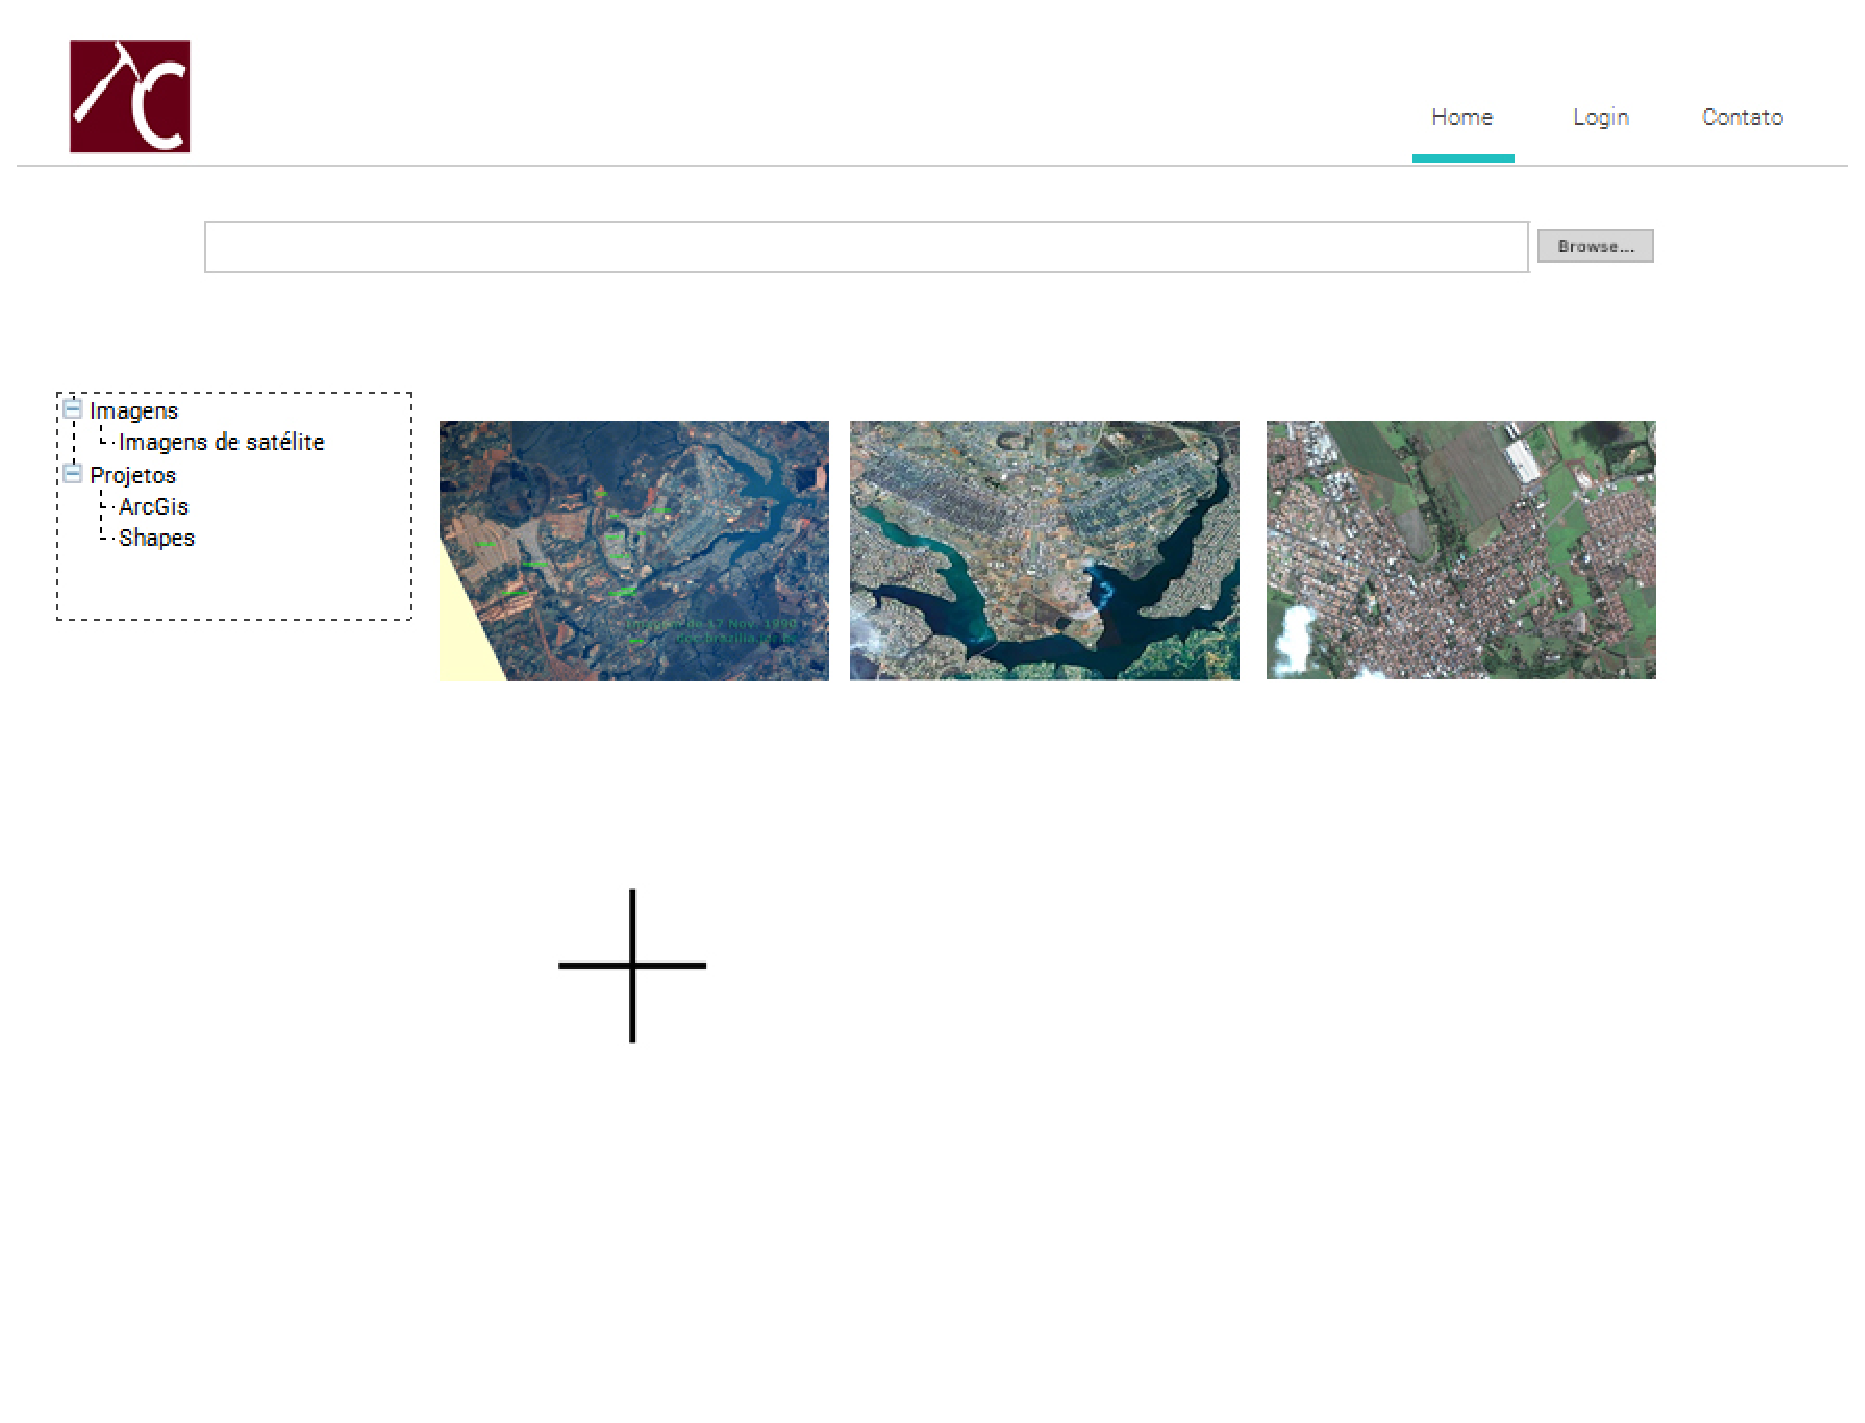
\includegraphics[width=10cm, keepaspectratio=false]{figuras/gerencia/pagina-upload.eps}
    \caption{Protótipo da página onde é realizado o upload de imagens de satélite ou projetos do ArcGis}
  \end{figure}

\subsection{Requisitos elicitados}

  \subsubsection{História de usuário 1}
    \textbf{Eu} como usuário, \textbf{desejo} salvar uma imagem de satélite. \textbf{Para que eu possa} acessar a qualquer momento e local posteriormente

    Prioridade: \textbf{Alta}

    Dificuldade: 5

  \subsubsection{História de usuário 2}

    \textbf{Eu} como usuário, \textbf{desejo} acessar uma imagem de satélite do banco. \textbf{Para que eu possa} realizar meu trabalho

    Prioridade: \textbf{Alta}

    Dificuldade: 3

  \subsubsection{História de usuário 3}

    \textbf{Eu} como usuário, \textbf{desejo} excluir uma imagem de satélite do banco. \textbf{Para que eu possa} organizar melhor meus arquivos

    Prioridade: \textbf{Média}

    Dificuldade: 3

  \subsubsection{História de usuário 4}
    \textbf{Eu} como usuário, \textbf{desejo} salvar um projeto ArcGIS. \textbf{Para que eu possa} acessar a qualquer momento e local posteriormente

    Prioridade: \textbf{Alta}

    Dificuldade: 8

  \subsubsection{História de usuário 5}
    \textbf{Eu} como usuário, \textbf{desejo} acessar um projeto ArcGIS. \textbf{Para que eu possa} realizar meu trabalho

    Prioridade: \textbf{Alta}

    Dificuldade: 5

  \subsubsection{História de usuário 6}
    \textbf{Eu} como usuário, \textbf{desejo} excluir um projeto ArcGIS. \textbf{Para que eu possa} organizar melhor meus arquivos

    Prioridade: \textbf{Alta}

    Dificuldade: 5

  \subsubsection{História de usuário 7}
    \textbf{Eu} como usuário, \textbf{desejo} alterar um projeto ArcGIS. \textbf{Para que eu possa} consertar possíveis erros

    Prioridade: \textbf{Baixa}

    Dificuldade: 5

  \subsubsection{História de usuário 8}
    \textbf{Eu} como desenvolvedor, \textbf{desejo} implementar um sistema de criptografia. \textbf{Para que eu possa} garantir segurança aos dados

    Prioridade: \textbf{Média}

    Dificuldade: 8

  \subsubsection{História de usuário 9}
    \textbf{Eu} como desenvolvedor, \textbf{desejo} implementar um sistema de validação de integridade dos arquivos. \textbf{Para que eu possa} garantir que os dados não sejam corrompidos 

    Prioridade: \textbf{Média}

    Dificuldade: 8

  \subsubsection{História de usuário 10}
    \textbf{Eu} como desenvolvedor, \textbf{desejo} implementar um sistema de backup. \textbf{Para que eu possa} garantir maior integridade ao banco

    Prioridade: \textbf{Média}

    Dificuldade: 8

  \subsubsection{História de usuário 11}
    \textbf{Eu} como administrador, \textbf{desejo} um sistema de permissões. \textbf{Para que eu possa} garantir acesso aos dados somente por autorizados 

    Prioridade: \textbf{Alta}

    Dificuldade: 8

  \subsubsection{História de usuário 12}
    \textbf{Eu} como usuário, \textbf{desejo} me cadastrar na ferramenta. \textbf{Para que eu possa} utilizar a mesma 

    Prioridade: \textbf{Alta}

    Dificuldade: 5

  \subsubsection{História de usuário 13}
    \textbf{Eu} como usuário, \textbf{desejo} editar meu perfil. \textbf{Para que eu possa} atualizar minhas informações

    Prioridade: \textbf{Média}

    Dificuldade: 5

  \subsubsection{História de usuário 14}
    \textbf{Eu} como administrador, \textbf{desejo} ser capaz de deletar perfis de usuário. \textbf{Para que eu possa} remover contas de usuário que não trabalham mais na empresa

    Prioridade: \textbf{Alta}

    Dificuldade: 3

  \subsubsection{História de usuário 15}
    \textbf{Eu} como administrador, \textbf{desejo} uma ferramenta de log. \textbf{Para que eu possa} acompanhar as atividade dos funcionários 

    Prioridade: \textbf{Média}

    Dificuldade: 8

  \subsubsection{História de usuário 16}
    \textbf{Eu} como usuário, \textbf{desejo} visualizar informações da imagem. \textbf{Para que eu possa} ter acesso a imagem específica que tenho interesse

    Prioridade: \textbf{Média}

    Dificuldade: 3

  \subsubsection{História de usuário 17}
    \textbf{Eu} como usuário, \textbf{desejo} visualizar informações do projeto. \textbf{Para que eu possa} ter acesso ao projeto específico que tenho interesse

    Prioridade: \textbf{Média}

    Dificuldade: 5

  \subsubsection{História de usuário 18}
    \textbf{Eu} como usuário, \textbf{desejo} poder criar pastas. \textbf{Para que eu possa} organizar da maneira que desejar meus projetos

    Prioridade: \textbf{Média}

    Dificuldade: 3

  \subsubsection{História de usuário 19}
    \textbf{Eu} como usuário, \textbf{desejo} renomear arquivos. \textbf{Para que eu possa} organizar da maneira que desejar meus projetos

    Prioridade: \textbf{Média}

    Dificuldade: 5

  \subsubsection{História de usuário 20}
    \textbf{Eu} como usuário, \textbf{desejo} mover arquivos. \textbf{Para que eu possa} organizar da maneira que desejar meus projetos

    Prioridade: \textbf{Média}

    Dificuldade: 5



\section{Gerência de mudança}

  Falar sobre o targetProcess, inserir algumas imagens, rastreabilidade e atributos dos requisitos e etc\ldots

  Em construção\ldots

\section{Rastreabilidade}

  Nesse tópico será apresentada a rastreabilidade vertical e horizontal dos requisitos elicitados.

\subsection{Rastreabilidade Vertical}

A rastreabilidade vertical pode ser percebida em “níveis” o mais alto e mais próximo do mundo real são os épicos, que são separadas em features e implementadas em histórias de usuário. A ferramenta Targetprocess apresenta essa rastreabilidade de uma maneira bastante simple e intuitiva. 

\begin{figure}[!htb]
    \centering
    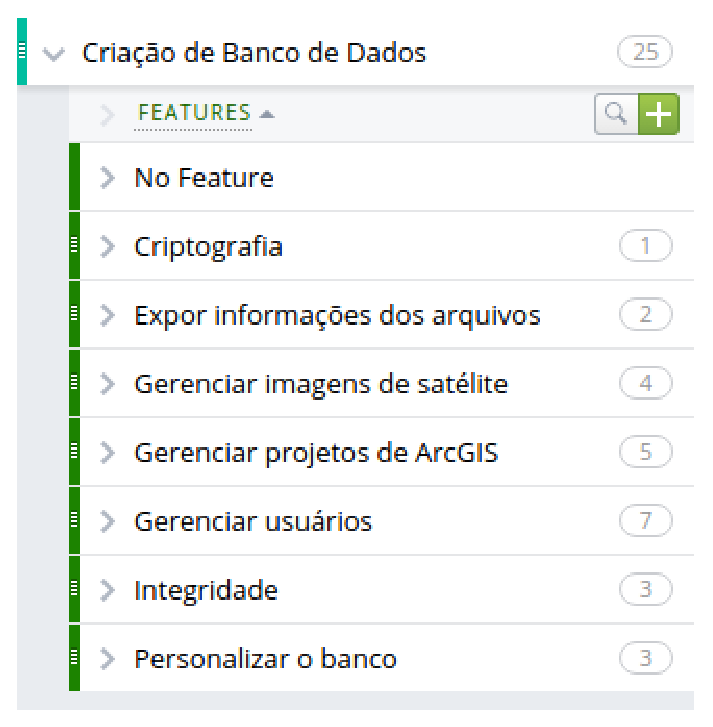
\includegraphics[width=10cm, keepaspectratio=false]{figuras/rastreabilidade/vertical/features.eps}
    \caption{Visão geral da rastreabilidade. O épico Criação de Banco e suas Features}
  \end{figure}

  \begin{figure}[!htb]
    \centering
    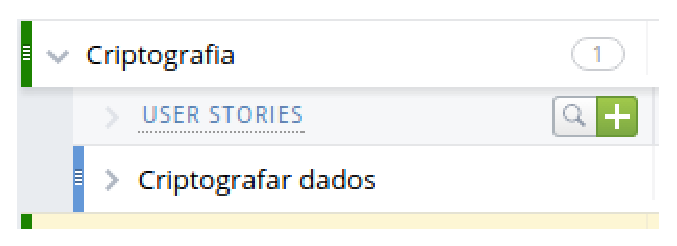
\includegraphics[width=10cm, keepaspectratio=false]{figuras/rastreabilidade/vertical/feature_criptografia.eps}
    \caption{Rastreabilidade vertical entre Épico Criação de Banco e a Feature Criptografia e sua História de Usuário Criptografar Dados}
  \end{figure}

  \begin{figure}[!htb]
    \centering
    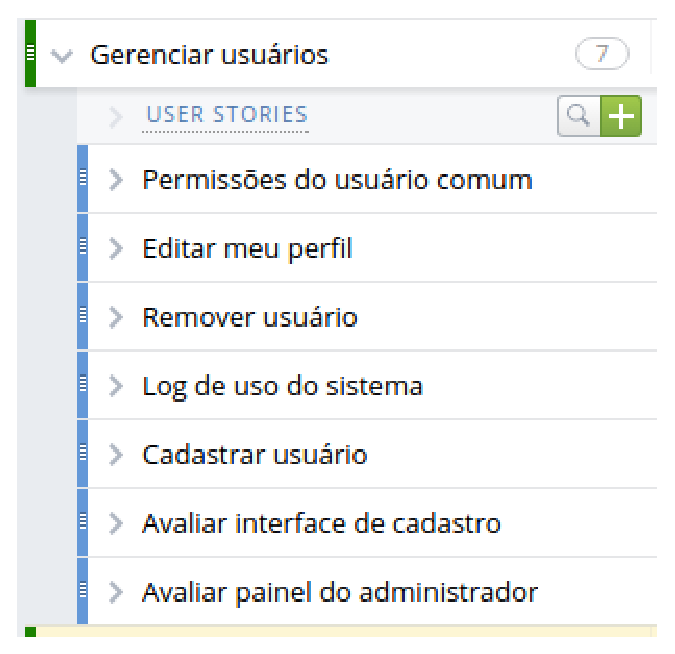
\includegraphics[width=10cm, keepaspectratio=false]{figuras/rastreabilidade/vertical/feature_gerenciar_usuario.eps}
    \caption{Rastreabilidade vertical entre Épico Criação de Banco e a Feature Gerenciar Usuário e suas História de Usuário}
  \end{figure}

  \begin{figure}[!htb]
    \centering
    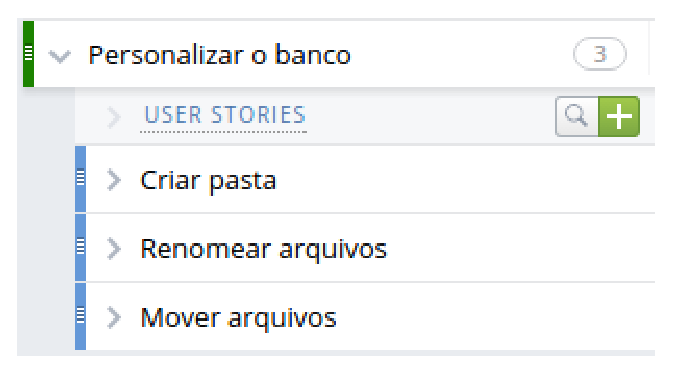
\includegraphics[width=10cm, keepaspectratio=false]{figuras/rastreabilidade/vertical/feature_personalizar_banco.eps}
    \caption{Rastreabilidade vertical entre Épico Criação de Banco e a Feature Personalizar Banco e suas História de Usuário}
  \end{figure}

  \begin{figure}[!htb]
    \centering
    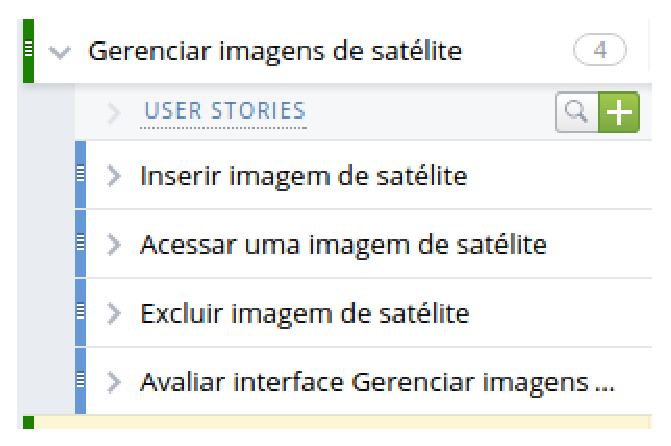
\includegraphics[width=10cm, keepaspectratio=false]{figuras/rastreabilidade/vertical/feature_gerenciar_imagens.eps}
    \caption{Rastreabilidade vertical entre Épico Criação de Banco e a Feature Gerenciar Imagens de Satélite e suas História de Usuário}
  \end{figure}

  \begin{figure}[!htb]
    \centering
    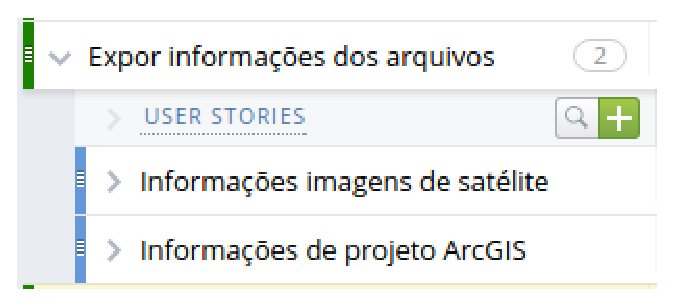
\includegraphics[width=10cm, keepaspectratio=false]{figuras/rastreabilidade/vertical/feature_expor.eps}
    \caption{Rastreabilidade vertical entre Épico Criação de Banco e a Feature Expor Informações dos Arquivos e suas História de Usuário}
  \end{figure}

  \begin{figure}[!htb]
    \centering
    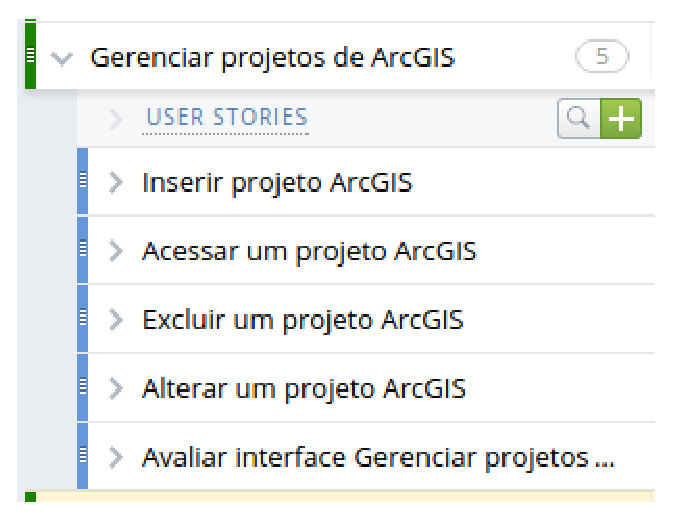
\includegraphics[width=10cm, keepaspectratio=false]{figuras/rastreabilidade/vertical/feature_gerenciar_projeto.eps}
    \caption{Rastreabilidade vertical entre Épico Criação de Banco e a Feature Gerenciar Projetos de ArcGIS e suas História de Usuário}
  \end{figure}

  \begin{figure}[!htb]
    \centering
    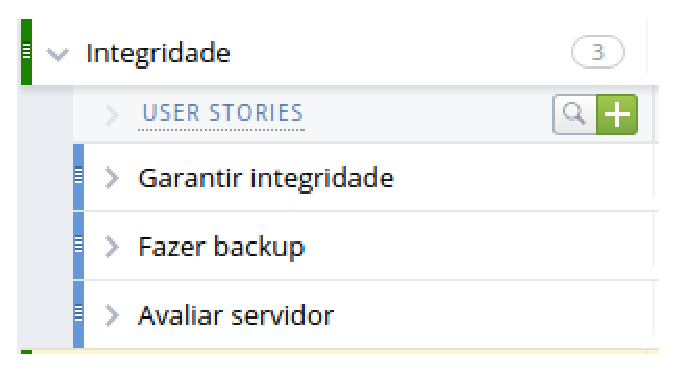
\includegraphics[width=10cm, keepaspectratio=false]{figuras/rastreabilidade/vertical/feature_integridade.eps}
    \caption{Rastreabilidade vertical entre Épico Criação de Banco e a Feature Integridade e suas História de Usuário}
  \end{figure}




\subsection{Rastreabilidade Horizontal}

